\documentclass[11pt,a4paper]{article}
\usepackage[T1]{fontenc}
\usepackage[utf8]{inputenc}
\usepackage{newtxtext,newtxmath}
\usepackage[a4paper,margin=24mm]{geometry}
\usepackage{cite,amsmath,graphicx,array,tabularx,booktabs,listings,xcolor,url,xurl,hyperref,microtype,enumitem,placeins}
\hypersetup{colorlinks=true,linkcolor=black,citecolor=black,urlcolor=blue,breaklinks=true,
 pdftitle={FungiCirno: Instance Segmentation and Cluster-Level Growth Monitoring of Oyster Mushrooms},
 pdfauthor={Nguyen Hai Nam; Nguyen Minh Thinh; Le Thien Khang}}
\urlstyle{same}
\setlength{\parskip}{0.22em}\setlength{\parindent}{1.2em}
\renewcommand{\arraystretch}{1.12}
\setlist[itemize]{leftmargin=1.5em,itemsep=0.12em,topsep=0.2em,parsep=0pt}
\setlist[enumerate]{leftmargin=1.7em,itemsep=0.12em,topsep=0.2em,parsep=0pt}
\emergencystretch=2.5em
\lstset{basicstyle=\ttfamily\small,columns=fullflexible,breaklines=true,keepspaces=true,showstringspaces=false,frame=single,rulecolor=\color{black!25},backgroundcolor=\color{black!2}}
\title{FungiCirno: Instance Segmentation and Cluster-Level Growth Monitoring of Oyster Mushrooms}
\author{Nguyen Hai Nam, Nguyen Minh Thinh, and Le Thien Khang\\
\small Project repository: \url{https://github.com/h-nam-sys/FungiCirno}}
\date{}
\begin{document}
\maketitle

\begin{abstract}
Monitoring oyster mushroom growth from time-lapse images requires more than detecting visible clusters in individual frames. The same cluster must be measured consistently over time, while missed detections and identity errors must remain distinguishable from actual changes in size. This study evaluates two instance-segmentation models for this task: a project implementation of Mask R-CNN with a ConvNeXt-Tiny feature pyramid and a fine-tuned YOLO26-L-seg model. The four-sequence \emph{Pleurotus ostreatus} dataset is divided by sequence into 1,728 training, 433 validation, and 528 test frames. On the test set, YOLO26-L-seg achieved mask AP50:95 of 89.02\%, compared with 57.03\% for the Mask R-CNN baseline. Its mean relative measurement errors were 4.21\% for area, 1.49\% for width, and 1.56\% for height across matched instances. For growth monitoring, 2,169 of 2,663 annotated test observations were associated with a predicted track that met a 90\% source-identity-purity requirement; the macro-average source-consistent coverage across 23 clusters was 82.45\%. Across 2,140 eligible adjacent transitions from 22 source identities, macro-averaged growth-direction agreement was 89.75\% at a 5\% stable-change deadband. Tracking results are retrospective because the test sequences were inspected during development. The findings support the use of instance masks for cluster-level image-space measurement, while showing that identity continuity remains a limiting factor in some histories.
\end{abstract}

\noindent\textbf{Keywords:} oyster mushroom, instance segmentation, cluster tracking, growth monitoring, image-space measurement, YOLO26, Mask R-CNN.

\section{Introduction}

\subsection{Problem Statement}

Oyster mushrooms (\emph{Pleurotus ostreatus}) emerge and develop in clusters whose visible shape, area, and overlap change over time. A single image can show where a cluster is located, but growth monitoring requires a reliable record of that cluster across multiple observations. If detections are missed or identities are switched, the resulting size history can misrepresent the biological object even when individual segmentation masks appear plausible.

This study treats an annotated mushroom cluster as the unit of analysis. For each time-lapse frame, the task is to obtain an instance mask and its geometric measurements. Across frames, observations are associated with persistent, sequence-scoped identities so that each cluster can be represented by a time-ordered size history. The study focuses on clusters as annotated in the source dataset; it does not attempt to separate the individual fruitbodies within a cluster.

\subsection{Motivation and Applications}

Cluster-level measurements can help describe how mushroom size changes during cultivation and can provide a basis for more detailed production monitoring. The practical challenge is that neighboring clusters may overlap as they expand, illumination can vary, and partial harvesting or withering can alter the visible region. A useful analysis must therefore distinguish a genuinely smaller mask from a missing observation and must account for identity errors when interpreting a trajectory.

The target substrate block is a static scene reference rather than a tracked object. Although the source study reports physical block dimensions, the present evaluation does not establish a validated substrate mask or camera calibration. The reported area, width, and height are consequently image-space quantities. The source maturity labels are also not inferred from size alone: the original study defines them using visible fruitbody characteristics, and the ordering of mean cluster area is not consistent across the validation and test subsets \cite{charisis}.

\subsection{Objectives and Contributions}

The work has two closely related research objectives. The first is to evaluate instance segmentation as a means of delineating individual mushroom clusters and supporting accurate geometric measurement. The second is to assess whether those measurements can be assembled into useful cluster-level histories through temporal identity association.

The study compares two available segmentation checkpoints on a common sequence-separated test set, measures area and bounding-box dimensions on matched instances, and evaluates a mask-IoU tracker against the persistent identities in the source annotations. It also examines low-confidence recovery and tests whether allowing a track to survive missed sampled observations changes identity continuity. The contribution is an empirical evaluation of segmentation and downstream growth-history quality on this dataset, rather than a claim to introduce the general idea of mushroom-cluster tracking, which has already been studied by Charisis et al. \cite{charisis}.

\section{Literature Review}

\subsection{Classical Approaches}

Thresholding and morphology provide simple ways to separate foreground regions from a background. Otsu's method selects a global intensity threshold by maximizing between-class variance \cite{otsu}. It is efficient, but a single threshold is vulnerable to illumination changes and to mushrooms whose intensity resembles the substrate. Morphological opening and closing can suppress small artifacts or repair local gaps, although their effect depends on the structuring element and may remove thin structures or join neighboring objects. Watershed segmentation can separate touching regions when suitable markers are available, but irregular textures and weak boundaries can make marker selection unstable \cite{watershed}. These methods are relevant alternatives, but they were not implemented as experimental baselines in this project.

\subsection{Learning-Based Approaches}

Mask R-CNN extends a region-based detector with a parallel mask-prediction branch, providing instance-level boundaries rather than only bounding boxes \cite{maskrcnn}. ConvNeXt revisits convolutional network design using choices informed by more recent vision architectures and has been used as a feature extractor for detection and segmentation \cite{convnext}. YOLO26 is a later Ultralytics model family that includes instance-segmentation variants; the large YOLO26-L-seg configuration is the challenger evaluated here \cite{yolo26docs}. These models provide different segmentation implementations for comparison, but the available checkpoints were not trained under a matched-budget protocol.

\subsection{Oyster Mushroom Tracking and Growth Measurement}

Charisis et al. developed a Mask R-CNN-based pipeline for segmenting and tracking oyster mushroom clusters in time-lapse images. Their method includes post-processing for background and harvesting artifacts, mask-based temporal association, and a relative-size estimate using the static substrate block as a reference \cite{charisis}. They report a ConvNeXt-based model with mAP of 0.876, mAR of 0.858, and an F1 value of 0.867, and report tracking MOTA values of 0.967 and 0.927 for the two test sequences. Their work is the closest prior study to the present task and establishes that segmentation, identity association, and growth visualization have already been investigated for this dataset.

\subsection{Positioning of This Study}

FungiCirno uses the same source dataset and a related cluster-level formulation, but the Mask R-CNN checkpoint is a TorchVision ConvNeXt-Tiny-FPN adaptation rather than the original MMDetection implementation. YOLO26-L-seg is a separately fine-tuned one-class model. The comparison aligns the test frames, source annotations, class-agnostic output representation, and measurement code as far as practical. It does not reproduce the filtering and tracking pipeline of Charisis et al.; published values are therefore used as context, not as results from a direct reimplementation.

\section{Methodology}

\subsection{Dataset and Split}

The dataset contains 6,382 RGB images of oyster mushroom clusters at a reported resolution of 6,080 by 3,420 pixels, collected in four time-lapse experiments. The source annotations contain 37,004 cluster instances and three maturity labels: \texttt{immature}, \texttt{well-defined}, and \texttt{overstayed} \cite{dataset,charisis}. Images were originally captured every 15 minutes. The source dataset is available from its Zenodo record (DOI: 10.5281/zenodo.15041243). The project does not redistribute the dataset; users must obtain it from the source record and follow the reuse terms stated there.

The canonical manifest contains 2,689 of the 6,382 source images. The split is sequence-based: sequences 2 and 4 provide training and validation data, while sequences 1 and 3 are reserved for testing. In sequence 2, the validation interval is the contiguous frame-index range 470--704; in sequence 4, it is 396--593. The immediately adjacent frames (469 and 705 in sequence 2; 395 and 594 in sequence 4) are omitted as guard frames. All other indexed frames in sequences 2 and 4 are assigned to training. The manifest therefore assigns 938 frames from sequence 2 and 790 from sequence 4 to training, and 235 and 198 frames, respectively, to validation.

For testing, the manifest selects every eighth source-frame index, starting at zero, from each held-out sequence. This gives 261 frames from sequence 1 (indices 0--2,080) and 267 from sequence 3 (indices 0--2,128). The remaining frames in those sequences are not used in model development or evaluation; this sampling preserves a nominal two-hour interval from the source capture cadence of 15 minutes. In total, 3,693 source images are absent from the canonical split: 3,689 unsampled frames from the two test sequences and the four guard frames around the validation intervals. These are the exclusions encoded by the manifest, rather than an additional image-quality filter. The resulting split counts are listed in Table~\ref{tab:split}.

\begin{table}[!htbp]
\centering\small
\caption{Sequence-level split used for the reported experiments.}
\label{tab:split}
\begin{tabular}{lrrrr}
\toprule
Sequence & Train & Validation & Test & Role \\
\midrule
1 & 0 & 0 & 261 & Test \\
2 & 938 & 235 & 0 & Train/validation \\
3 & 0 & 0 & 267 & Test \\
4 & 790 & 198 & 0 & Train/validation \\
\midrule
Total & 1,728 & 433 & 528 & \\
\bottomrule
\end{tabular}
\end{table}

The source annotations contain an explicit \texttt{tracking\_id}; a COCO annotation ID alone is only an annotation-record identifier and is not treated as a persistent cluster identity. The audit verified all 6,084 ground-truth observations in the validation and test subsets against the tracked source JSON files. The full source contains 43 identities across its four sequences, and 40 occur in the evaluated validation/test subset. The test sequences contain 23 source identities. The compound keys used for evaluation are $(\texttt{SEQUENCE\_ID},\texttt{COCO\_ANNOTATION\_ID})$ for annotation records and $(\texttt{SEQUENCE\_ID},\texttt{tracking\_id})$ for physical cluster identity.

\subsection{Experimental Evaluation Workflow}

Both segmentation models are evaluated on the same validation and test frames. Their predictions are converted to a common class-agnostic cluster representation and compared with the source masks. One-to-one matched instances provide the basis for area and bounding-box measurements. YOLO26-L-seg predictions are also passed through the temporal association procedure; the resulting predicted tracks are joined to the source identities to assess continuity and construct per-cluster growth histories.

\subsection{Baseline: Mask R-CNN with ConvNeXt-Tiny-FPN}

The baseline is a project implementation of Mask R-CNN with a ConvNeXt-Tiny backbone and feature pyramid network. It is implemented with TorchVision and was trained with the three maturity-specific output classes in the source annotations. For the shared instance-segmentation evaluation, its output labels are collapsed to a single cluster category after inference. This makes the evaluation class-agnostic, but does not make its training objective identical to the one-class YOLO model. The retained experiment artifacts identify the evaluated checkpoint and inference configuration but do not preserve a complete Mask R-CNN training recipe, so its epoch count, optimizer, learning-rate schedule, and augmentation settings are not reported here.

The source images are high resolution, and pasting all predicted ROI masks into full-resolution image tensors on the GPU caused excessive memory use. The executed inference notebook therefore retains TorchVision's box resizing and ROI processing but pastes each full-resolution mask individually on the CPU using \texttt{paste\_masks\_in\_image}. A parity check against the corresponding TorchVision operation passed. This changes the location of mask pasting, not the model weights or the predicted ROI values \cite{pytorch,torchvision}.

\subsection{Comparison Method: YOLO26-L-seg}

YOLO26-L-seg was initialized from pretrained weights and fine-tuned for a single foreground class, \texttt{mushroom\_cluster} \cite{yolo26docs}. The run used 1,024-pixel input images, MuSGD optimization, an initial learning rate of 0.00038, momentum of 0.948, weight decay of 0.00027, and a maximum of 100 epochs with early stopping. Training stopped after 79 epochs. The checkpoint used in the final evaluation was epoch 30; it had been selected using validation aggregate-area error during checkpoint screening, not by selecting the highest validation mask AP. The historical aggregate-area result itself is not used as a reported result in this paper.

The source masks were converted to YOLO segmentation polygons by decoding the COCO representation, extracting external contours, and writing normalized polygon coordinates. The conversion retained the largest external contour for each annotation. Smaller disconnected components, where present, were therefore not represented in the YOLO training polygon. This is a known difference between the converted training target and the complete source mask.

At inference, YOLO26-L-seg used 1,024-pixel input, a candidate confidence floor of 0.001, NMS IoU of 0.70 with the default Ultralytics NMS mode, a maximum of 1,000 detections, and retina masks, with one frame processed per call. Mask R-CNN used a score floor of 0.001 and a maximum of 100 detections per frame. Its predicted masks were binarized at 0.50 after full-resolution mask pasting. These candidate-generation settings are distinct from the higher confidence thresholds selected on validation for fixed-threshold evaluation.

\subsection{Temporal Association and Cluster Measurement}

For two binary masks $M_i$ and $M_j$, the association similarity is intersection over union:
\begin{equation}
\operatorname{IoU}(M_i,M_j)=\frac{|M_i\cap M_j|}{|M_i\cup M_j|}.
\end{equation}
The tracker constructs a cost matrix $C_{ij}=1-\operatorname{IoU}(M_i,M_j)$ between active tracks and current detections and uses one-to-one assignment to obtain candidate matches. Pairs below an IoU threshold of 0.10 are rejected. The selected configuration uses a high-confidence threshold of 0.871056 and a second recovery stage with a minimum confidence of 0.60. Low-confidence detections can update an existing track but cannot initialize a new one. The selected maximum gap is zero sampled frames; a track that is not matched in the next sampled frame is closed. IDs are not recycled within a sequence.

For each observed mask $M_t$, area is the number of foreground pixels:
\begin{equation}
A_{\mathrm{px}}(t)=\sum_{x,y}M_t(x,y).
\end{equation}
Width and height are measured from the tight bounding box around the mask. For matched prediction/ground-truth pairs, absolute and relative errors are calculated separately for area, width, and height. A missing detection is not represented as a zero-area measurement. When a track has valid observations at two nominal times, its area change can be summarized as $[A(t_2)-A(t_1)]/(t_2-t_1)$. Raw capture timestamps were unavailable for the 961 evaluated frames, so the reported time axes use the nominal two-hour sampling interval rather than timestamp measurements.

A descriptive relative-size index is also calculated from training annotations. The reference area is the mean mask area of 3,365 training observations labeled \texttt{mature\_cluster}, corresponding to the source \texttt{well-defined} category, and equals $669{,}444.16\,\mathrm{px}^2$. For an observed cluster,
\begin{equation}
I_{\mathrm{size}}(t)=100\frac{A_{\mathrm{cluster}}(t)}{669{,}444.16}.
\end{equation}
The index is not capped at 100\%. It provides a common image-space reference for comparing cluster areas; it is not a maturity probability or harvest-readiness classifier. The source maturity categories are based on fruitbody characteristics, not size alone \cite{charisis}.

\subsection{Self-Implemented Core Algorithm}

The project implements the rectangular Hungarian assignment procedure from scratch for minimum-cost one-to-one matching. When the cost matrix has more rows than columns, the implementation transposes it, solves the smaller-row case, and maps the assignment back. The solver uses row and column potentials and predecessor links to find and augment a minimum-cost assignment. The core procedure is summarized below.

\begin{lstlisting}[caption={Rectangular Hungarian assignment used for track-to-detection association.},label={lst:hungarian}]
HUNGARIAN(C):
    if C has zero rows or columns: return empty assignment
    if rows(C) > columns(C):
        return transpose(HUNGARIAN(transpose(C)))

    initialize row potentials u, column potentials v
    initialize column matching p and predecessor links way

    for each row i:
        attach row i to the dummy column 0
        set all unused-column reduced costs to infinity
        repeat:
            mark current column j0 as used
            i0 = row currently assigned to j0
            find unused column j1 with minimum reduced cost:
                cur = C[i0,j] - u[i0] - v[j]
                update minv[j] and way[j] when cur is smaller
            delta = minimum minv[j] over unused columns
            update potentials for used columns by delta
            subtract delta from unused minv values
            j0 = j1
        until j0 is an unmatched column

        follow way links backward to augment the matching

    return all matched (row, column) pairs
\end{lstlisting}

The returned assignment is filtered by the tracker using the 0.10 mask-IoU acceptance threshold. The solver was compared with SciPy's \texttt{linear\_sum\_assignment} on 508 generated and hand-constructed cost matrices. Verification checked assignment validity and optimal total cost, allowing different pair order when multiple optimal assignments existed \cite{kuhn,scipy}. This test supports the implementation on the tested cases; it is not a proof for every possible input.

\section{Experiments and Results}

\subsection{Experimental Setup and Metrics}

Both models underwent fresh forward-pass inference on all 433 validation and 528 test frames; the evaluation did not reuse the earlier prediction cache. Fixed-threshold precision, recall, and operating-point F1 use confidence thresholds selected on validation: 0.871056 for YOLO26-L-seg and 0.757535 for Mask R-CNN. Ranked mask AP and AR were calculated with COCO evaluation over IoU thresholds from 0.50 to 0.95 in 0.05 increments, with a maximum of 100 detections per image \cite{coco}. Fixed-threshold metrics use one-to-one mask matching at IoU 0.50. Geometry errors are conditional on matched instances. Tracking is assessed against sequence-scoped source identities using IDF1, identity switches, fragmentation, and MOTA computed from the equation used by Charisis et al.; the underlying frame matching is the project's mask-IoU matching at 0.50. The candidate-generation settings are reported in Section 3.4; the validation-selected thresholds are applied only when calculating fixed-threshold metrics.

\subsection{Segmentation Results and Comparison with Charisis et al.}

Table~\ref{tab:segmentation} reports the principal segmentation results. YOLO26-L-seg achieved higher AP at both individual thresholds and across the COCO IoU range. Its precision at the validation-selected operating threshold was also substantially higher. Mask R-CNN achieved higher recall at its own selected threshold, but this came with many more false positives. The comparison is between the available project checkpoints, not a controlled comparison of training budgets or identical class objectives.

\begin{table}[!htbp]
\centering\scriptsize
\caption{Test segmentation metrics and published Charisis reference. The harmonic mAP--mAR value is distinct from fixed-threshold operating-point F1.}
\label{tab:segmentation}
\resizebox{\linewidth}{!}{%
\begin{tabular}{lrrrrrrrr}
\toprule
System & mAP & AP50 & AP75 & mAR@100 & H(mAP,mAR) & Precision & Recall & F1$_{op}$ \\
\midrule
YOLO26-L-seg & 89.02 & 96.21 & 94.72 & 91.86 & 90.42 & 99.31 & 85.99 & 92.17 \\
Mask R-CNN + ConvNeXt & 57.03 & 72.38 & 66.97 & 83.77 & 67.86 & 58.21 & 93.09 & 71.63 \\
Charisis et al. (published) & 87.60 & -- & -- & 85.80 & 86.70 & -- & -- & -- \\
\bottomrule
\end{tabular}%
}
\end{table}

The published ConvNeXt result from Charisis et al. is close to YOLO26-L-seg in mAP and lower in mAR under the summary values available in the paper. This is a contextual comparison, not evidence that FungiCirno reproduces or exceeds the original pipeline. In particular, the present mAR is COCO AR@100; the cited Charisis metric description specifies averaging over IoU thresholds but does not state the same maximum-detection setting. Their MMDetection implementation and filtering pipeline are also not reproduced here. The harmonic value in the table is $2\,\mathrm{mAP}\,\mathrm{mAR}/(\mathrm{mAP}+\mathrm{mAR})$, following the mAP--mAR construction used for the Charisis F1; it should not be confused with the conventional precision--recall F1 at a selected confidence threshold.

\begin{figure}[!htbp]
\centering
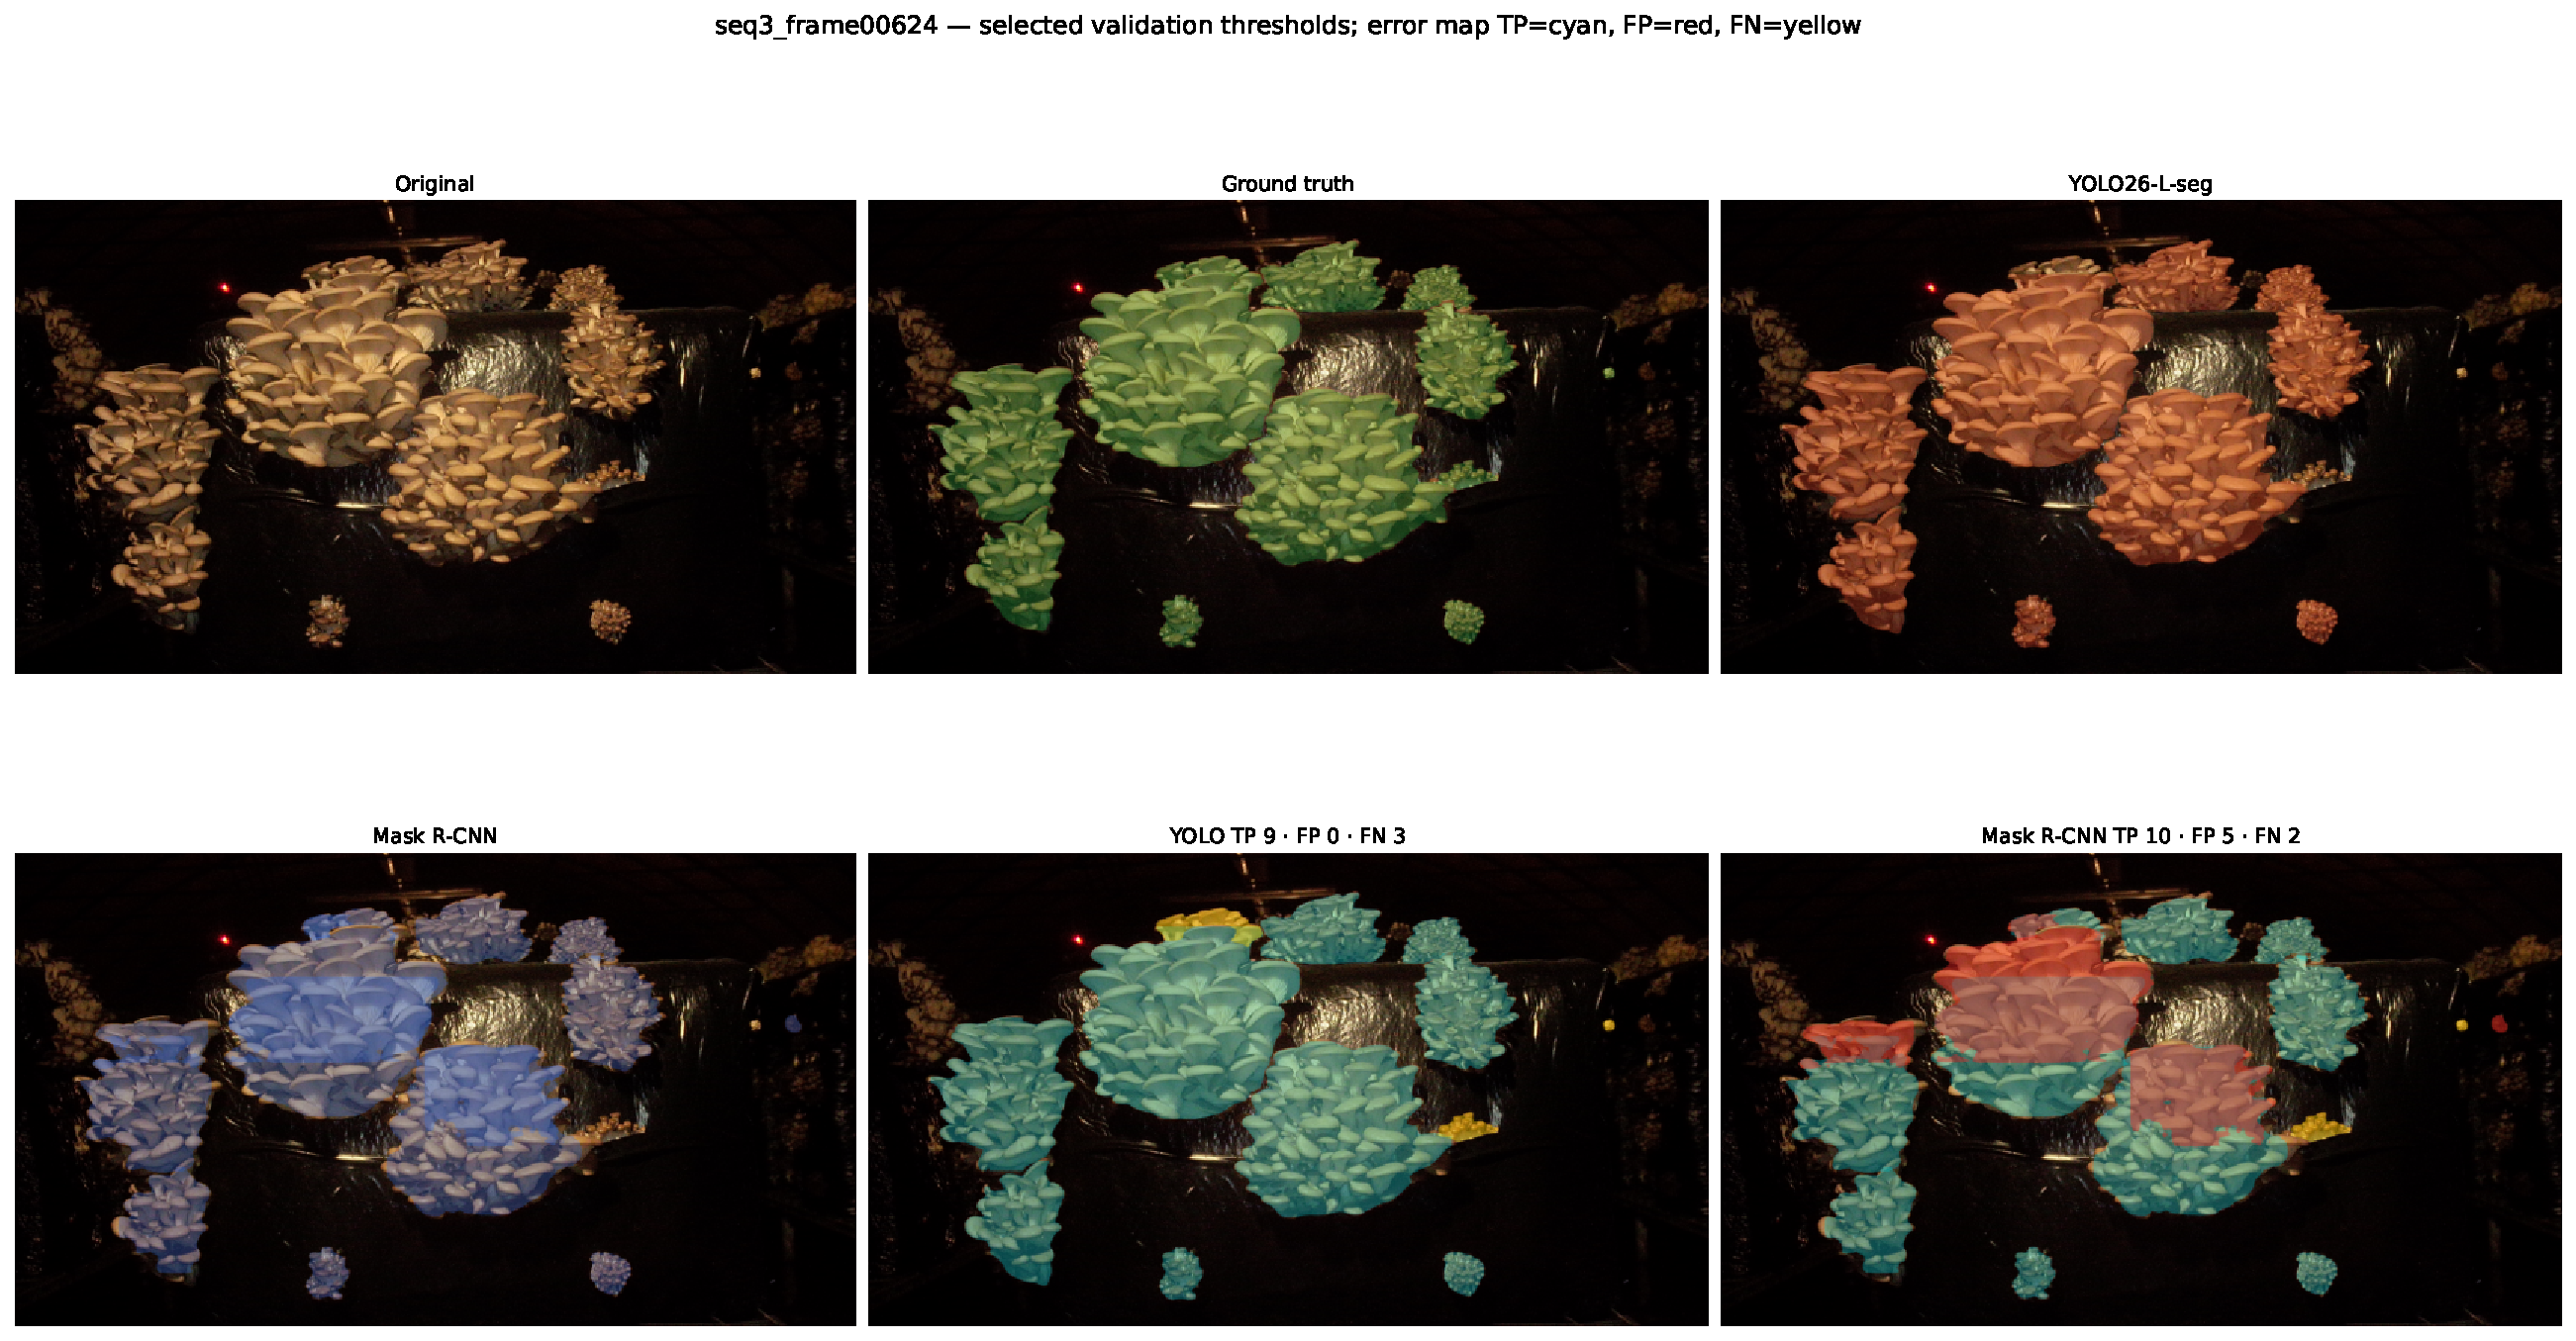
\includegraphics[width=0.99\linewidth]{figures/qualitative_hard_test.pdf}
\caption{Difficult test example (sequence 3, frame 624). The six panels show the original frame, source masks, both model predictions, and TP/FP/FN error maps. YOLO26-L-seg produced 9 TP, 0 FP, and 3 FN; Mask R-CNN produced 10 TP, 5 FP, and 2 FN at their respective validation-selected thresholds.}
\label{fig:qualitative-hard}
\end{figure}

\begin{figure}[!htbp]
\centering
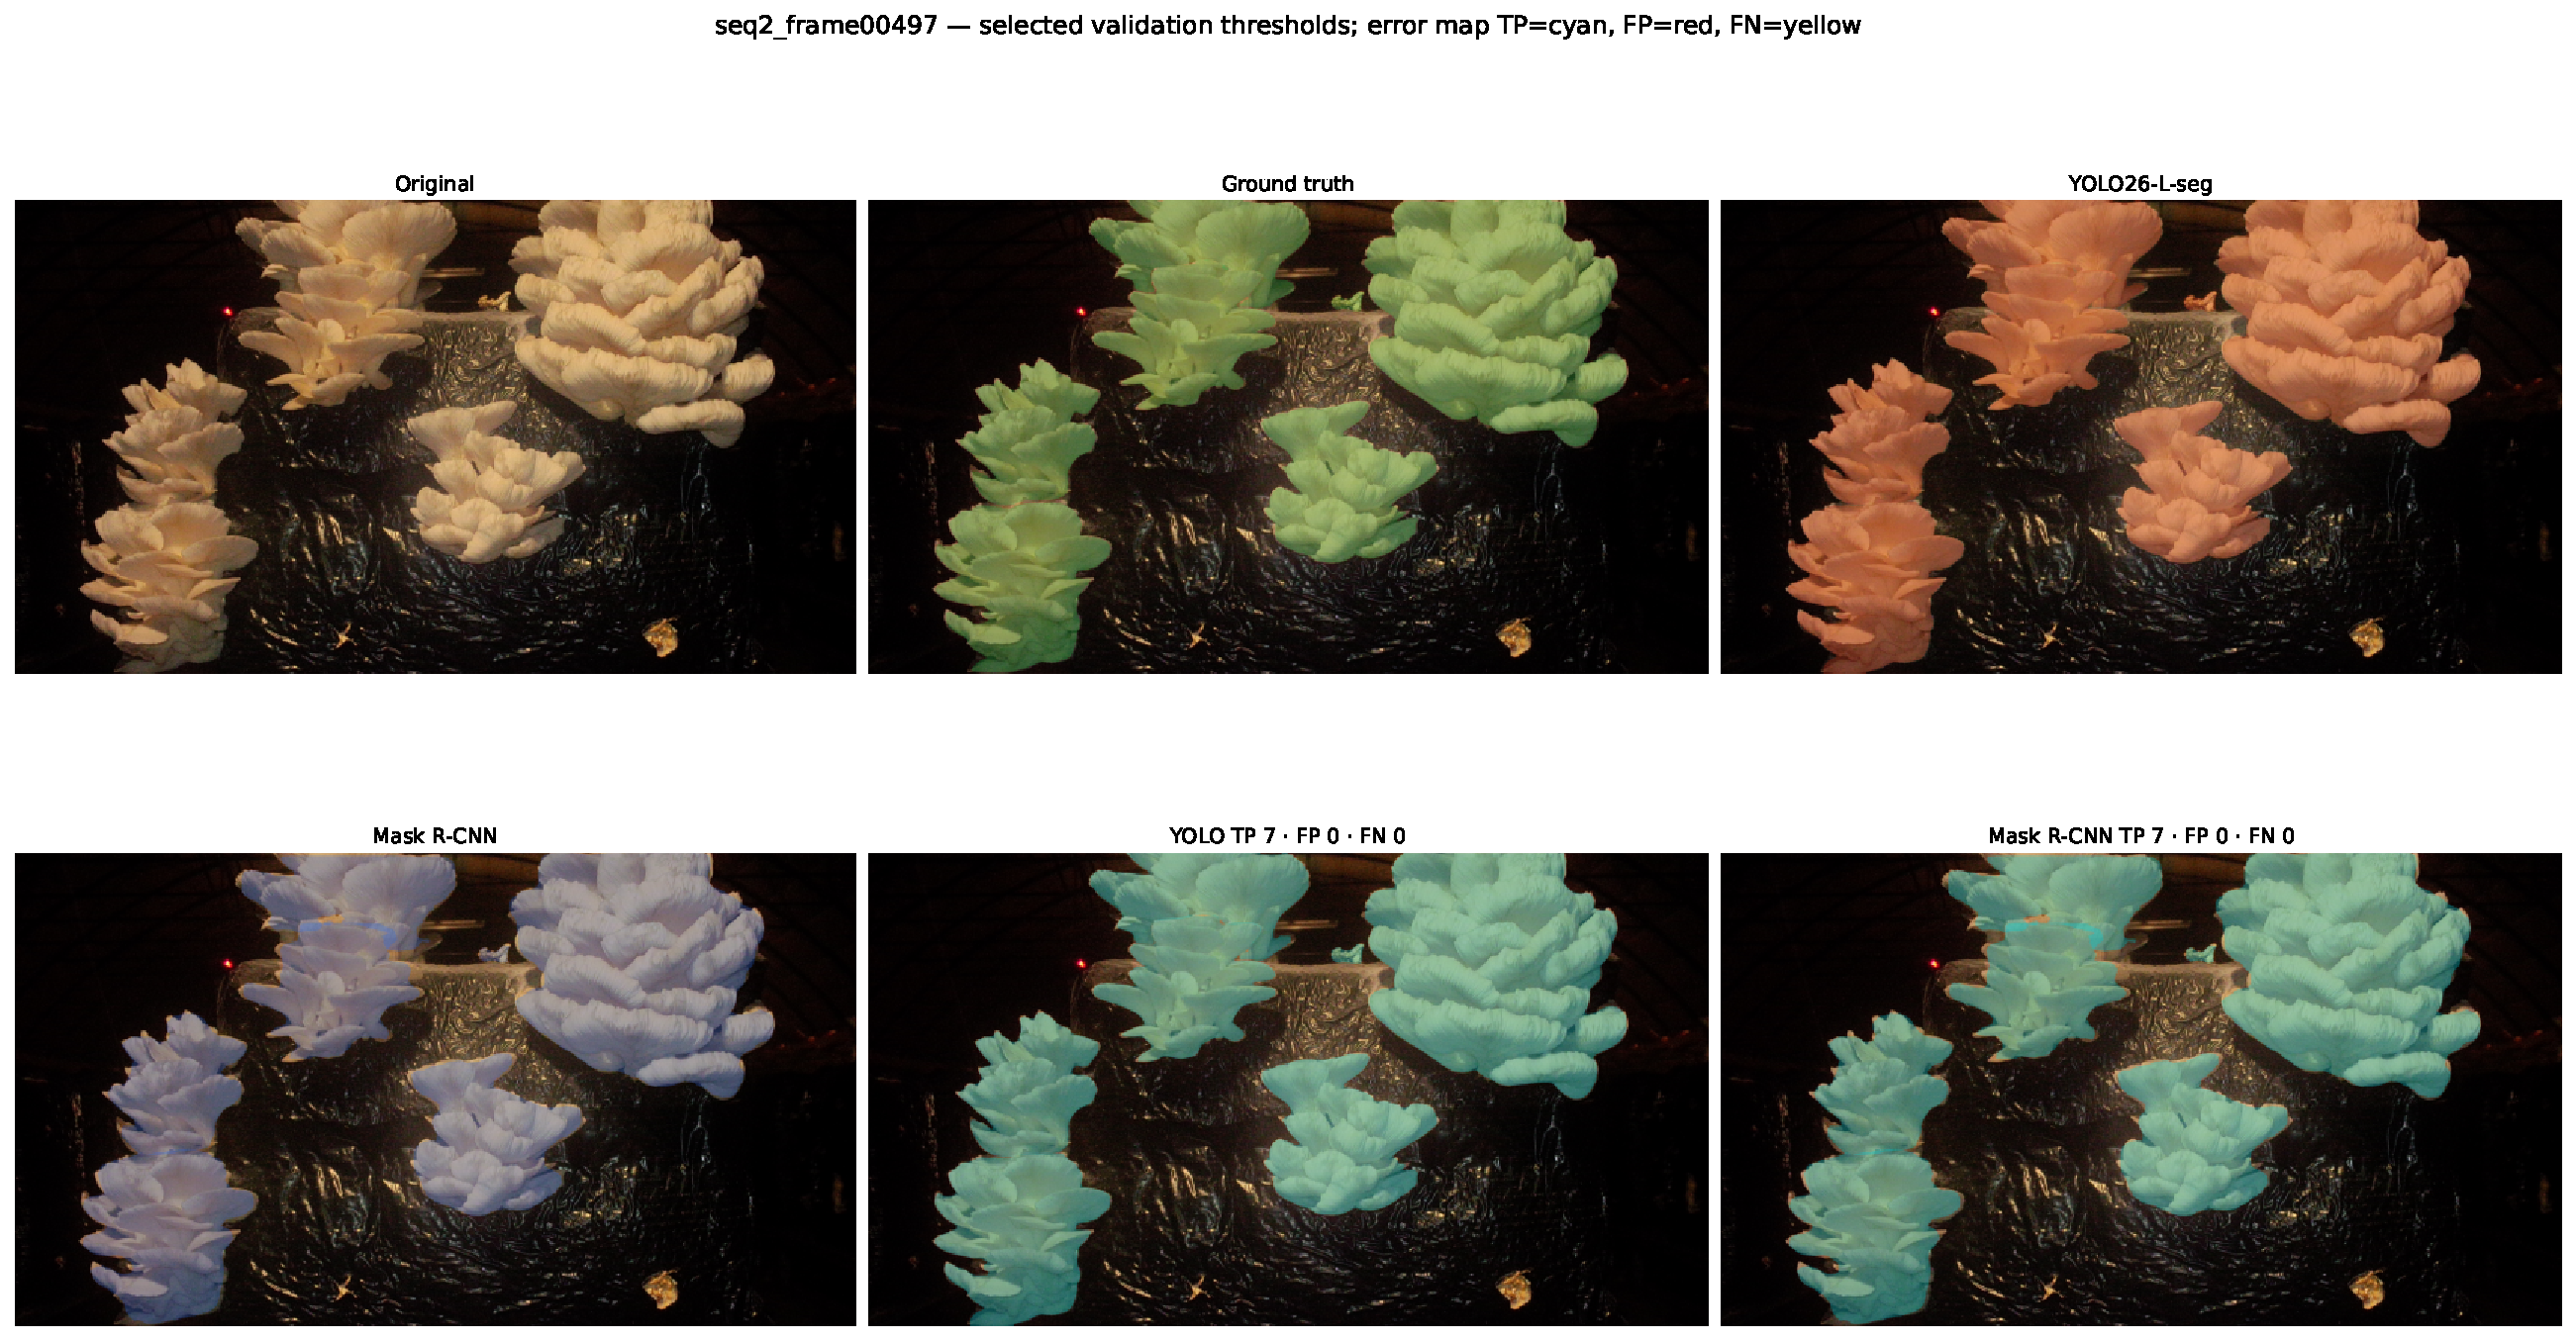
\includegraphics[width=0.99\linewidth]{figures/qualitative_clean_validation.pdf}
\caption{Clean validation example (sequence 2, frame 497). Both models matched the seven annotated clusters without false positives or missed instances at their respective selected thresholds.}
\label{fig:qualitative-clean}
\end{figure}
\FloatBarrier

\subsection{Per-Cluster Measurement Accuracy}

Segmentation quality matters here because mask errors propagate directly into area and bounding-box measurements. Predictions were matched one-to-one to ground-truth masks within each frame at IoU 0.50. For each measurement $m$ (area, width, or height), the mean relative absolute error is computed over the $N$ matched pairs as
\begin{equation}
\operatorname{RAE}_{m}=\frac{100}{N}\sum_{i=1}^{N}\frac{|\hat{m}_{i}-m_{i}|}{m_{i}},
\label{eq:rae}
\end{equation}
where $\hat{m}_{i}$ is the predicted value and $m_i$ is the corresponding ground-truth value. The table reports errors only for matched pairs; detection recall remains necessary to understand how many clusters were missed. YOLO26-L-seg had lower mean relative absolute error for all three measurements. Its area RAE was 4.21\%, compared with 6.96\% for Mask R-CNN, while the width and height errors were also smaller.

\begin{table}[!htbp]
\centering\small
\caption{Per-instance measurement errors on matched test instances. MAE is in image-space pixels or pixels squared; RAE is the mean per-instance relative absolute error.}
\label{tab:measurement}
\begin{tabular}{llrrr}
\toprule
Measurement & Model & Matched $n$ & MAE & RAE \\
\midrule
Area (px$^2$) & YOLO26-L-seg & 2,290 & 10,918.30 & 4.21\% \\
Area (px$^2$) & Mask R-CNN & 2,479 & 33,286.18 & 6.96\% \\
Width (px) & YOLO26-L-seg & 2,290 & 9.46 & 1.49\% \\
Width (px) & Mask R-CNN & 2,479 & 43.25 & 5.63\% \\
Height (px) & YOLO26-L-seg & 2,290 & 8.94 & 1.56\% \\
Height (px) & Mask R-CNN & 2,479 & 47.67 & 7.42\% \\
\bottomrule
\end{tabular}
\end{table}

\begin{figure}[!htbp]
\centering
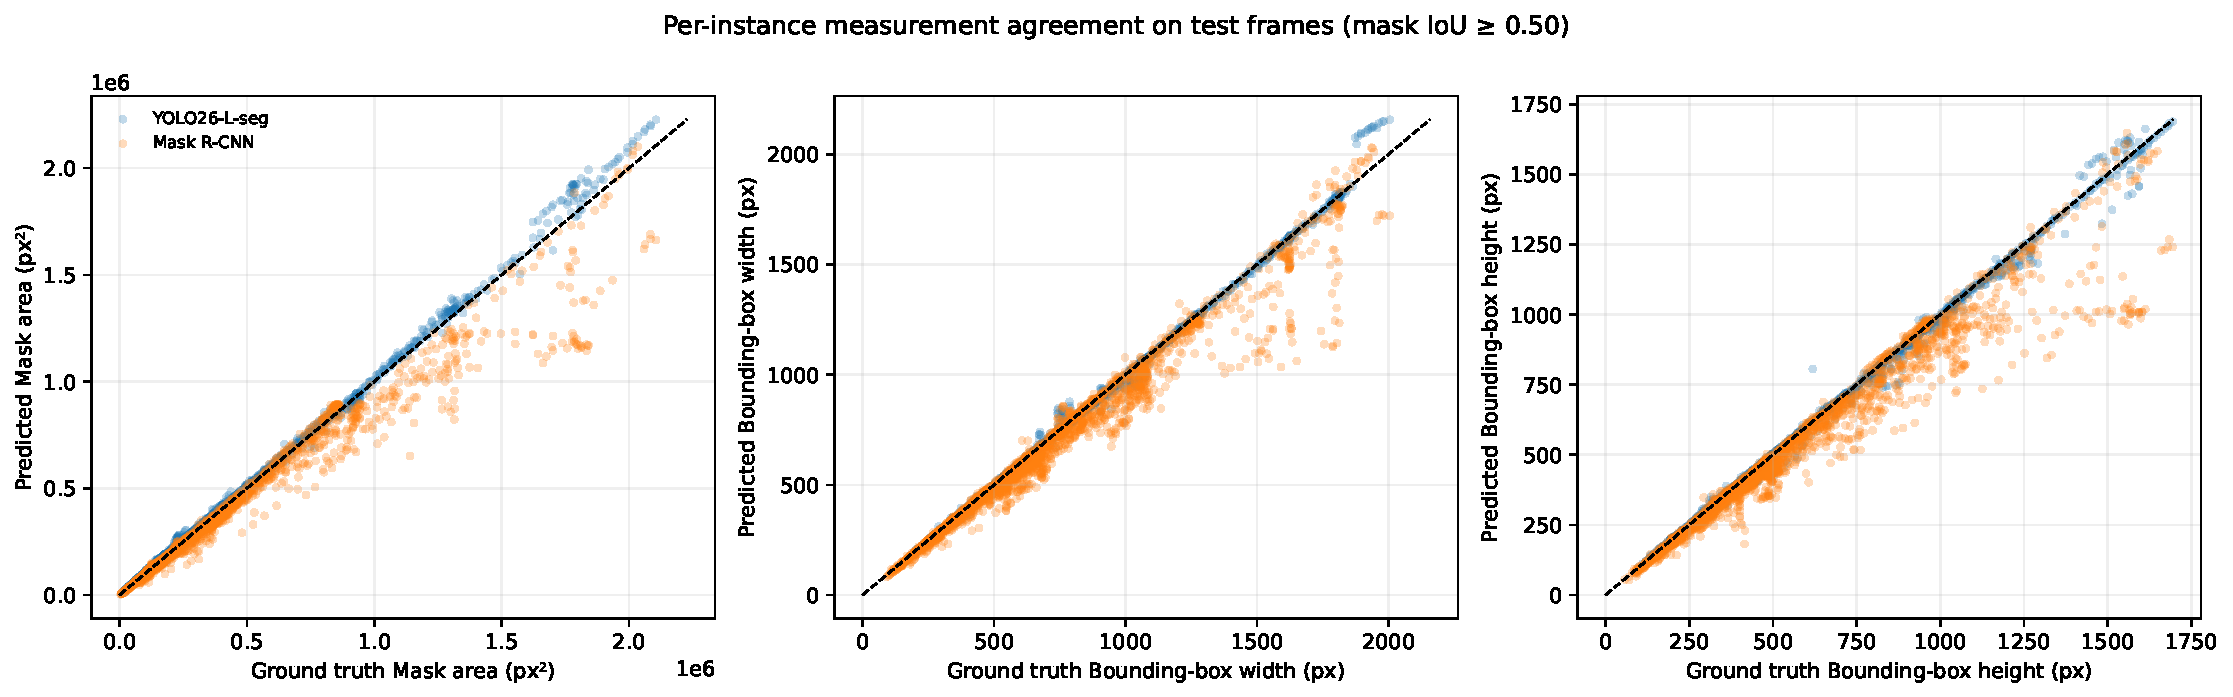
\includegraphics[width=0.95\linewidth]{figures/measurement_agreement.pdf}
\caption{Ground-truth versus predicted area, width, and height for matched test instances. The diagonal represents perfect agreement.}
\label{fig:measurement-agreement}
\end{figure}

\subsection{Temporal Tracking and Growth-History Monitoring}

The source annotations provide persistent identities for 23 clusters in the test sequences, covering 2,663 ground-truth observations. With the selected zero-gap tracker, 2,415 observations were matched to predictions (90.69\% pooled observation coverage). A stricter analysis counted a match as source-consistent only when the predicted track's dominant source identity was the same as the ground-truth identity and its purity was at least 90\%. This left 2,169 source-consistent observations: 81.45\% of all test annotations when pooled, or 82.45\% when coverage is first calculated for each identity and then averaged equally across the 23 identities. The latter macro-average prevents long-lived clusters from dominating the summary.

Five source identities were split across multiple predicted tracks. In addition, one predicted track in sequence 3 combined observations from two source identities. Of its 246 matched observations, 154 belonged to the dominant identity and 92 to a second identity, giving a track purity of 62.60\%. Purity is calculated over the complete predicted track, and the 90\% requirement is applied at the track level before observations enter the strict history analysis. Because this track falls below the threshold, all 246 observations associated with it are excluded, not only the 92 observations belonging to the secondary identity. This removes the entire mixed track from the strict source-consistent count, leaving 2,169 observations from the 2,415 ordinary matches. Figure~\ref{fig:history-coverage} shows the resulting coverage by source identity, and Figure~\ref{fig:mixed-purity} details the mixed predicted track.

\begin{table}[!htbp]
\centering\small
\caption{Summary of source-identity-aware growth-history evaluation on the test sequences.}
\label{tab:growth-summary}
\begin{tabular}{lr}
\toprule
Measure & Result \\
\midrule
Source identities / GT observations & 23 / 2,663 \\
Ordinary matched observations & 2,415 (90.69\% pooled) \\
Source-consistent observations & 2,169 (81.45\% pooled) \\
Macro source-consistent history coverage & 82.45\% \\
Identities with fragmented predicted histories & 5 of 23 \\
Strict adjacent transitions / identities & 2,140 / 22 \\
Area RAE within strict histories & 4.36\% \\
Width RAE within strict histories & 1.54\% \\
Height RAE within strict histories & 1.65\% \\
Trend agreement at 5\% deadband & 89.75\% \\
\bottomrule
\end{tabular}
\end{table}

\begin{figure}[!htbp]
\centering
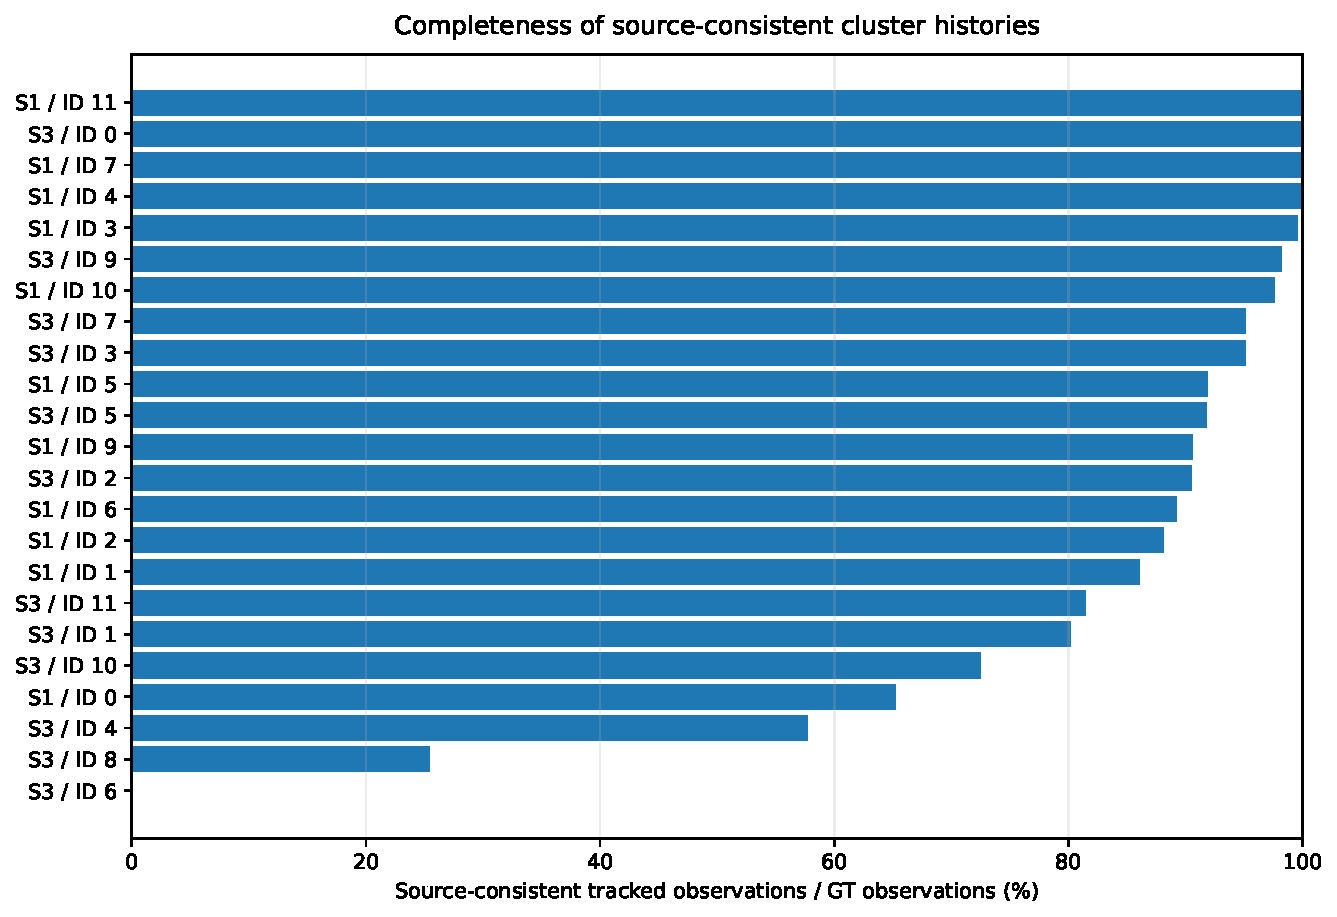
\includegraphics[width=0.92\linewidth]{figures/history_coverage.pdf}
\caption{Source-consistent observation coverage for each of the 23 test identities. An observation is counted only when it is assigned to a predicted track whose dominant source identity agrees and whose track purity is at least 90\%.}
\label{fig:history-coverage}
\end{figure}

For the strict histories, area, width, and height RAE were 4.36\%, 1.54\%, and 1.65\%, respectively. These values are calculated only over source-consistent matched observations and are therefore not interchangeable with the all-matched geometry results in Table~\ref{tab:measurement}. Growth direction was evaluated only between adjacent held-out samples whose two endpoints were both matched to the same predicted track. No missing observation was interpolated. There were 2,140 eligible adjacent transitions across 22 source identities. At a 5\% stable-change deadband, macro-averaged growth-direction agreement was 89.75\%: agreement was calculated within each eligible identity first and then averaged equally across the 22 identities. The result depends on the deadband: agreement was 87.07\%, 82.36\%, 89.75\%, and 94.03\% for deadbands of 0\%, 2\%, 5\%, and 10\%, respectively.

\begin{figure}[!htbp]
\centering
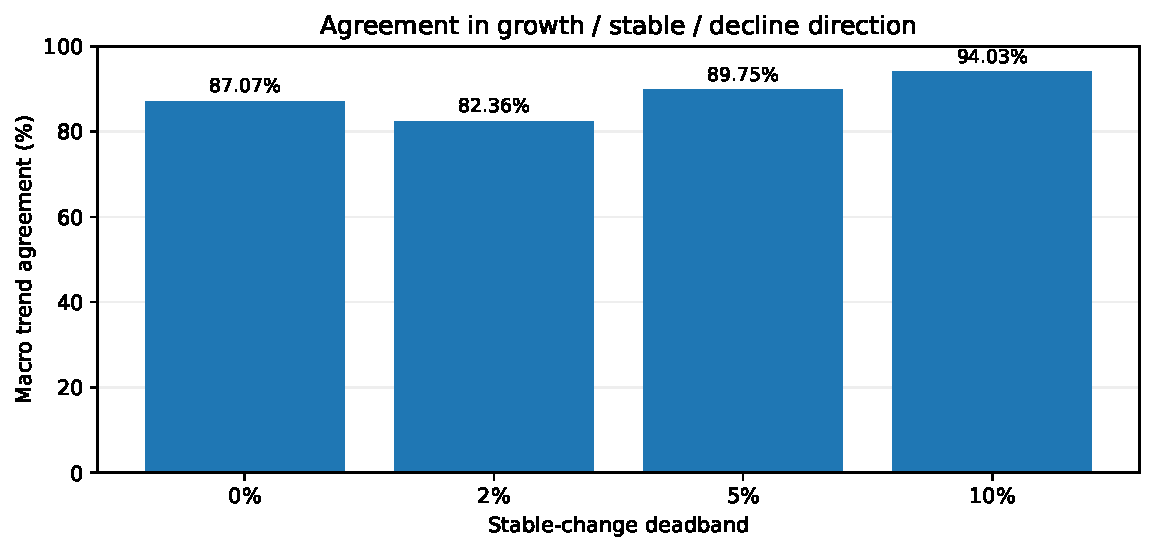
\includegraphics[width=0.77\linewidth]{figures/growth_trend_sensitivity.pdf}
\caption{Sensitivity of growth-direction agreement to the relative-change deadband. The metric is macro-averaged over identities with eligible adjacent, same-track transitions; the deadband changes which small changes are classified as stable.}
\label{fig:trend-sensitivity}
\end{figure}

The area history in Figure~\ref{fig:growth-area} illustrates a successful long sequence. Sequence 1, source identity 3, has 252 source-consistent observations represented by one predicted track. The predicted area follows the broad rise, peak, and decline in the ground-truth trajectory. Figure~\ref{fig:growth-normalized} shows the same record relative to its first observation, while Figure~\ref{fig:cluster-progression} shows four corresponding image crops at selected times. These examples demonstrate what a continuous history can represent; they do not imply that every source identity receives an equally complete track.

\begin{figure}[!htbp]
\centering
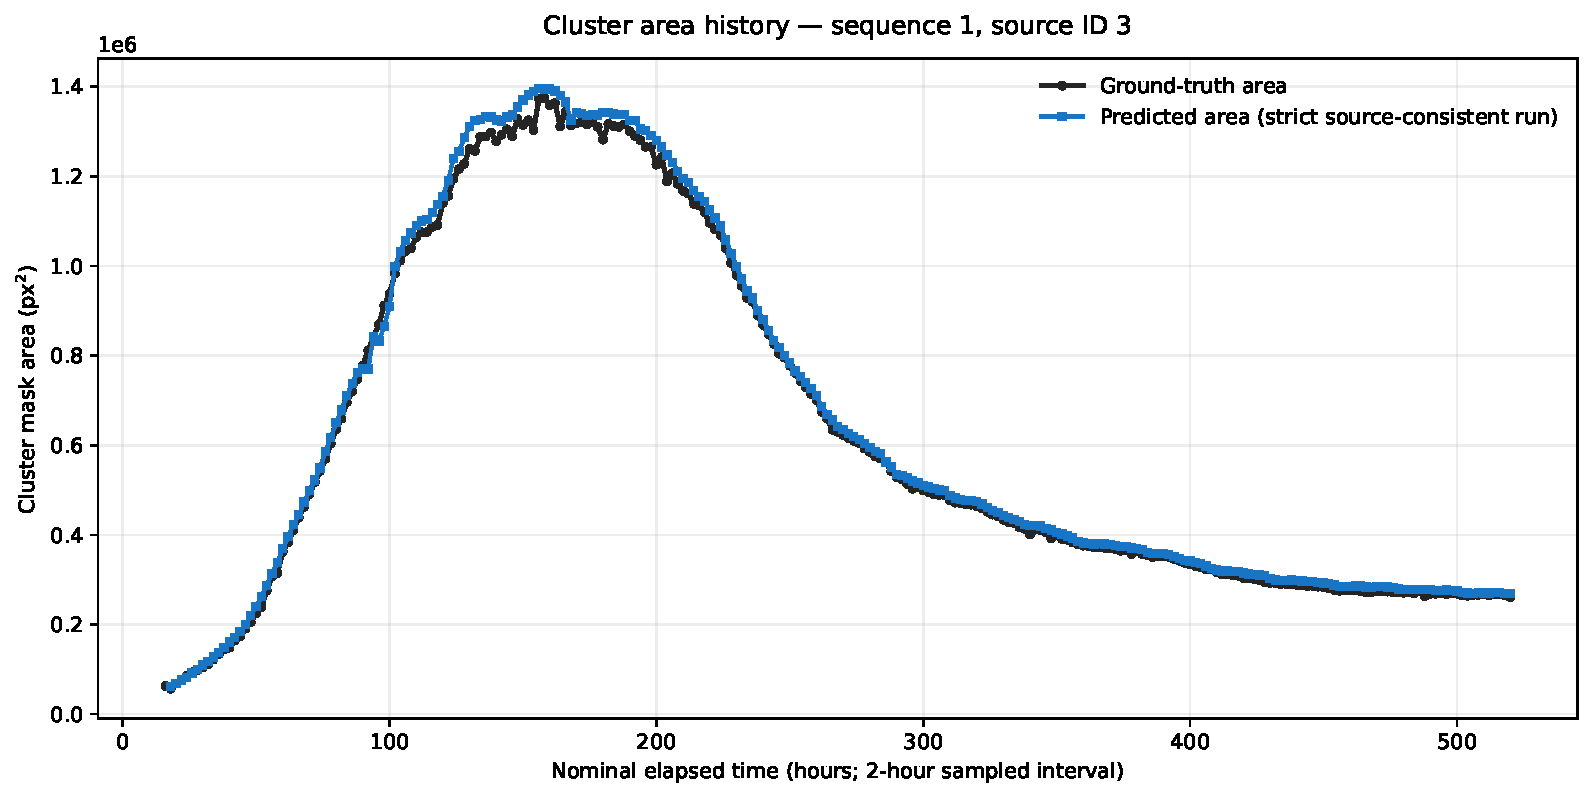
\includegraphics[width=0.92\linewidth]{figures/growth_history_area.pdf}
\caption{Ground-truth and predicted image-space area for sequence 1, source identity 3, over 252 source-consistent observations. The time axis is nominal, derived from the two-hour sampling interval.}
\label{fig:growth-area}
\end{figure}

\begin{figure}[!htbp]
\centering
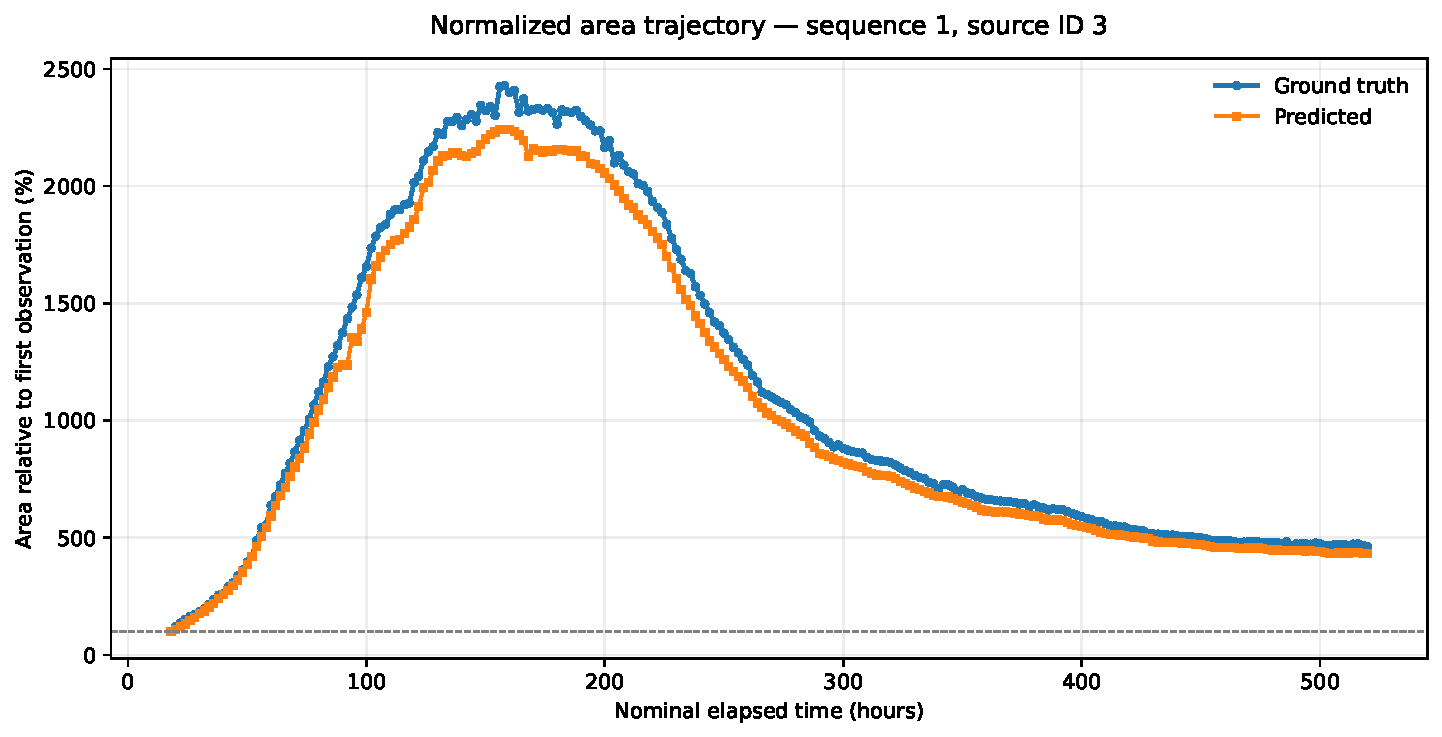
\includegraphics[width=0.92\linewidth]{figures/growth_history_normalized.pdf}
\caption{The same sequence 1 history normalized to the first valid observation. The curve shows relative image-space area, not a biological maturity scale.}
\label{fig:growth-normalized}
\end{figure}

\begin{figure}[!htbp]
\centering
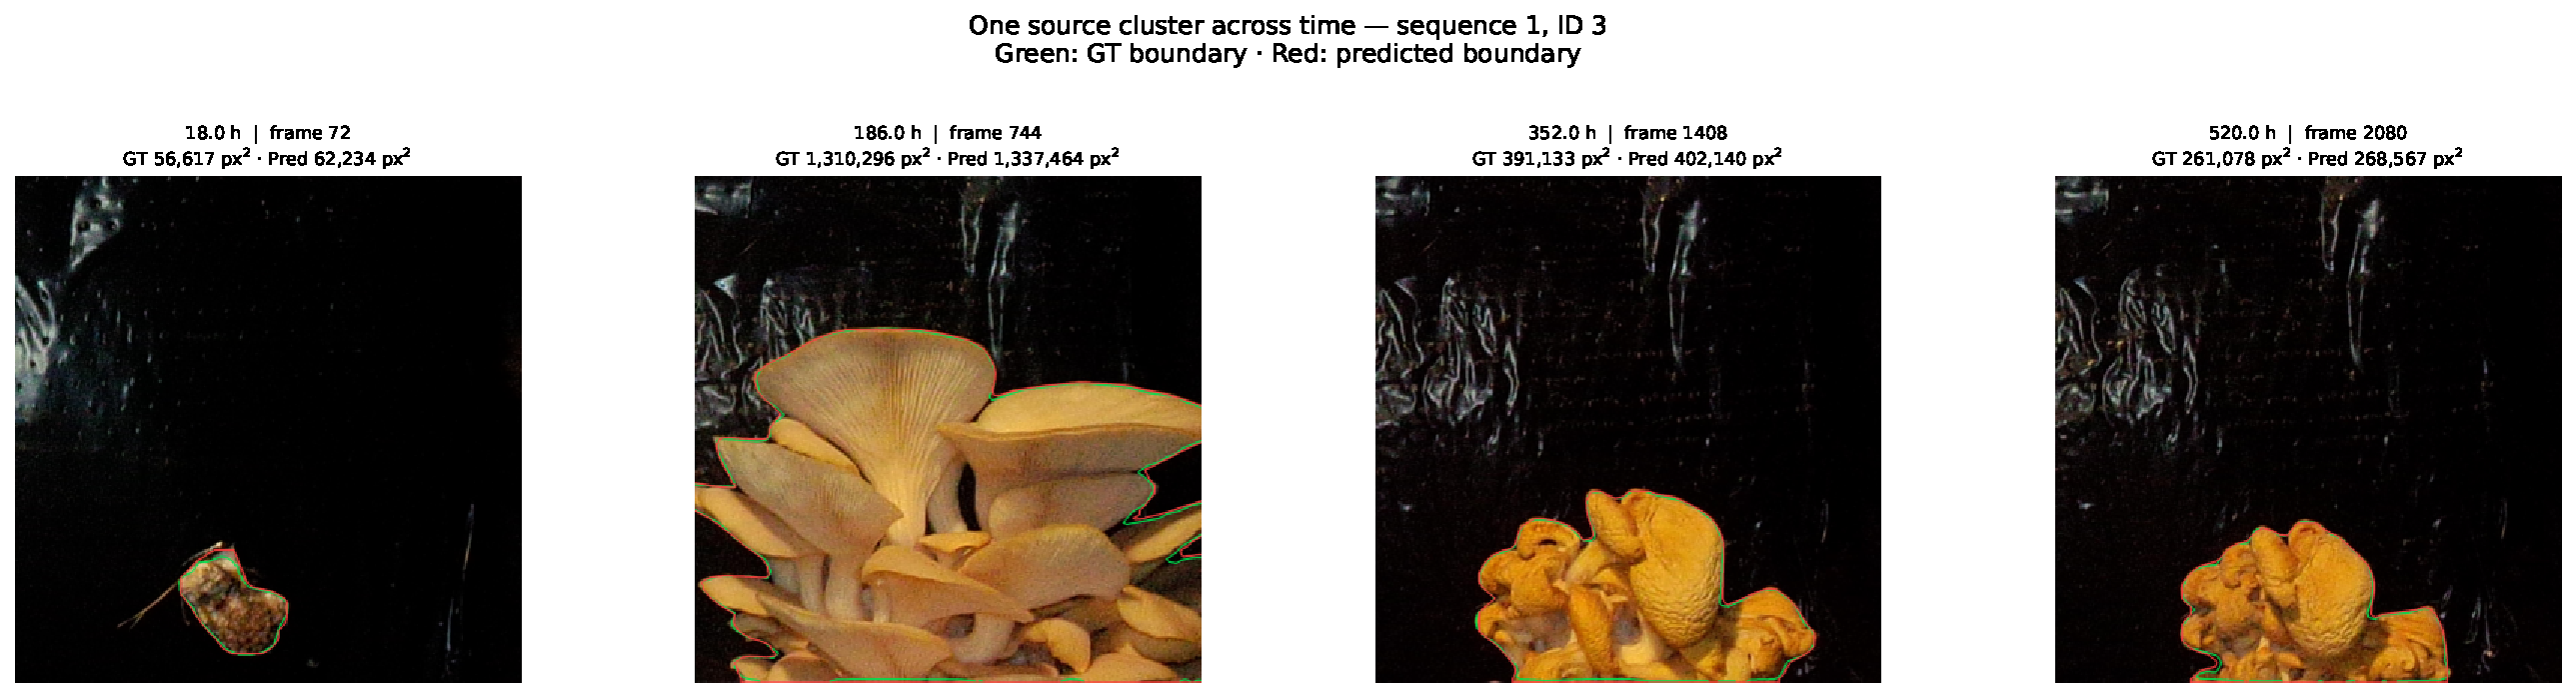
\includegraphics[width=0.99\linewidth]{figures/cluster_progression.pdf}
\caption{Four chronological observations of sequence 1, source identity 3. Green and red outlines denote the source mask and predicted mask, respectively. The selected observations are not consecutive; their nominal elapsed times are shown above each crop.}
\label{fig:cluster-progression}
\end{figure}

\begin{figure}[!htbp]
\centering
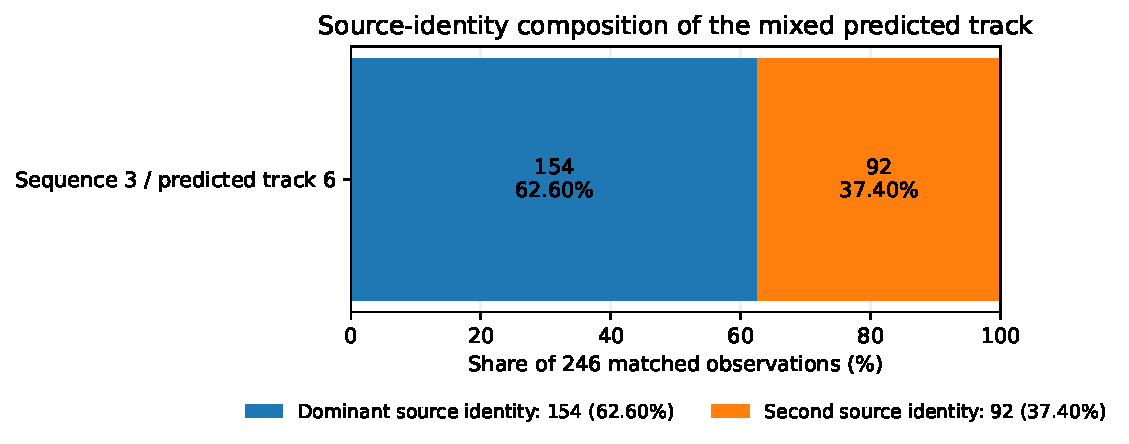
\includegraphics[width=0.68\linewidth]{figures/mixed_identity_purity.pdf}
\caption{Identity composition of sequence 3, predicted track 6. Of 246 matched observations, 154 (62.60\%) belong to the dominant source identity and 92 (37.40\%) belong to a second source identity.}
\label{fig:mixed-purity}
\end{figure}
\FloatBarrier

\subsection{Tracking Ablation and Comparison with Charisis et al.}

The four-way ablation isolates mask-IoU association, centroid-distance gating, and low-confidence recovery. Low-confidence recovery was restricted to updating existing tracks and did not create new tracks. It produced the largest change in this retrospective test analysis. Adding the centroid gate did not produce a consistent benefit: it slightly changed IDF1 but increased identity switches and fragmentation relative to the recovery-only configuration.

\begin{table}[!htbp]
\centering\small
\caption{Retrospective tracker ablation on the test sequences. MOTA uses the Charisis equation with the project's frame-level matching; it is not a reproduction of their full tracking pipeline.}
\label{tab:tracking-ablation}
\begin{tabular}{lrrrrr}
\toprule
Configuration & IDF1 & MOTA & IDSW & Fragmented GT IDs & Frag. events \\
\midrule
IoU only (A) & 74.30\% & 83.29\% & 56 & 11 & 56 \\
Spatial only (B) & 76.47\% & 83.03\% & 63 & 12 & 56 \\
IoU + recovery (C) & 85.56\% & 89.19\% & 6 & 5 & 6 \\
Spatial + recovery (D) & 85.87\% & 88.77\% & 15 & 8 & 8 \\
\bottomrule
\end{tabular}
\end{table}

MOTA was recalculated per test sequence using the published equation $1-(FP+FN+IDS)/GT$. With the selected zero-gap tracker, sequence 1 produced 971 TP, 11 FP, 43 FN, and 1 identity switch; sequence 3 produced 1,444 TP, 23 FP, 205 FN, and 5 identity switches. The corresponding MOTA values are shown beside the Charisis published references in Table~\ref{tab:mota-charisis}. The lower values, particularly for sequence 3, indicate that identity association remains a significant limitation. The equation is aligned, but the frame matching, tracker, and filtering procedure are not the same as in the original work.

\begin{table}[!htbp]
\centering\small
\caption{Sequence-level MOTA calculated with the Charisis equation and compared with the published values.}
\label{tab:mota-charisis}
\begin{tabular}{lrrrrrr}
\toprule
Sequence & GT & TP & FP & FN & FungiCirno MOTA & Charisis MOTA \\
\midrule
1 & 1,014 & 971 & 11 & 43 & 94.58\% & 96.70\% \\
3 & 1,649 & 1,444 & 23 & 205 & 85.87\% & 92.70\% \\
\bottomrule
\end{tabular}
\end{table}

The maximum-gap sensitivity test considered gaps of zero, one, or two missed sampled observations. All three settings produced identical validation metrics across the eight disjoint validation streams. The tie-break rule therefore selected the smallest gap (zero). On the already-inspected test sequences, gap one increased IDF1 from 85.56\% to 88.56\% and MOTA from 89.19\% to 89.75\%; gap two gave IDF1 of 88.26\% and MOTA of 89.34\%. These test results are retrospective and were not used to select the reported tracker configuration.

\begin{table}[!htbp]
\centering\small
\caption{Validation tie and retrospective test sensitivity to the maximum number of missed sampled observations.}
\label{tab:gap-sensitivity}
\begin{tabular}{rrrrrr}
\toprule
Max gap & Validation IDF1 & Test IDF1 & Test MOTA & Test IDSW & Test coverage \\
\midrule
0 & 99.88\% & 85.56\% & 89.19\% & 6 & 90.69\% \\
1 & 99.88\% & 88.56\% & 89.75\% & 2 & 91.21\% \\
2 & 99.88\% & 88.26\% & 89.34\% & 2 & 91.33\% \\
\bottomrule
\end{tabular}
\end{table}

\subsection{Runtime and Memory}

Both models were evaluated on an NVIDIA Tesla T4. In the latest full run, mean inference-call time was 156.09 ms per frame for YOLO26-L-seg and 344.41 ms for Mask R-CNN; mean mask-export times were 1,258.92 ms and 5,085.54 ms, respectively. Peak host resident memory was 2,551.86 MiB for YOLO26-L-seg and 2,627.89 MiB for Mask R-CNN. Across the combined run, peak CUDA allocation was 1.03 GiB and peak reserved memory was 1.25 GiB. The timers have different boundaries: the YOLO timer includes the synchronized Ultralytics prediction call, while the Mask R-CNN timer covers its model forward and ROI/box post-processing. The mask-export stages also perform different work. These measurements describe the recorded implementation and should not be interpreted as a controlled speed ranking.

\begin{table}[!htbp]
\centering\small
\caption{Runtime and memory measurements from the fresh Tesla T4 evaluation. Timing boundaries differ by model.}
\label{tab:runtime}
\resizebox{\linewidth}{!}{%
\begin{tabular}{lrrrr}
\toprule
Model & Inference mean (ms) & Inference p95 (ms) & Mask export mean (ms) & Peak host RSS (MiB) \\
\midrule
YOLO26-L-seg & 156.09 & 161.14 & 1,258.92 & 2,551.86 \\
Mask R-CNN + ConvNeXt & 344.41 & 386.10 & 5,085.54 & 2,627.89 \\
\bottomrule
\end{tabular}%
}
\end{table}

\section{Discussion}

The segmentation comparison favors YOLO26-L-seg on the available checkpoints. Its advantage is not limited to mask AP: the lower area, width, and height errors show that the difference carries through to measurements on matched instances. The Mask R-CNN baseline has higher recall at its selected threshold, but its lower precision reflects a much larger number of false positives. The results therefore support YOLO26-L-seg as the stronger segmentation model for this particular class-agnostic evaluation, not as a universal replacement for Mask R-CNN.

The growth-history analysis shows why segmentation quality and temporal identity must be evaluated together. The selected tracker matched 90.69\% of test observations when pooled, but only 81.45\% of all annotations were assigned to a source-consistent track under the 90\% purity rule. Five source identities were fragmented, and one predicted track mixed two source identities. A long, accurate-looking trajectory can therefore coexist with identity failures elsewhere in the sequence. The 252-observation sequence 1 example demonstrates that the method can preserve a useful area history, while the sequence 3 mixed track shows that this behavior is not uniform.

Low-confidence recovery was the most influential component in the four-way tracker ablation. The centroid-distance gate did not improve the overall identity measures consistently. The gap experiment suggests that retaining a track across a missed sampled observation may help, but validation could not distinguish the tested gap settings and the better gap-one test score is retrospective. A new, untouched sequence is needed before treating that result as evidence of general improvement.

\subsection{Error Analysis}

The dominant tracking failure in the refined audit is not a mask-quality error alone. In sequence 3, predicted track 6 contains observations from two source identities, with 62.60\% purity. Such a merge can create a plausible but incorrect growth history if it is not checked against source identity. Fragmentation creates the opposite problem: one source identity is represented by multiple predicted tracks, shortening or splitting its history. The strict history analysis addresses these errors by requiring a dominant source identity and at least 90\% track purity before using a predicted track for source-consistent growth measurement.

At the frame level, the difficult qualitative example shows missed YOLO instances and false positives from the Mask R-CNN baseline. These errors affect subsequent area measurements and can also interrupt temporal association. The clean validation example shows that both models can segment a frame well; the aggregate and history results indicate that performance across a sequence is more demanding than success on an individual image.

\subsection{Limitations}

The evaluation uses one species and four time-lapse sequences from one published dataset. Although test frames were held out from model training, the test sequences were inspected during tracker development; tracking and gap-sensitivity results are therefore retrospective. The reported MOTA uses the Charisis equation with the project's own frame matching, not the complete original tracking pipeline or a TrackEval implementation. The Mask R-CNN checkpoint is also a TorchVision adaptation rather than the original MMDetection model.

Test frames are sampled every two hours, although the source camera captured images every fifteen minutes. The tracker uses a zero-gap setting for the selected configuration and therefore closes a track after a missed sampled observation. Raw capture timestamps are unavailable, so growth plots use nominal time. Measurements remain two-dimensional pixel area and bounding-box dimensions; no physical calibration, volume, mass, or harvest-readiness estimate is claimed. Finally, the relative-size index is a reference to the training mean area of the source \texttt{well-defined} category, not a maturity classifier.

\subsection{Future Work}

The most direct improvement is to evaluate track persistence over missed observations on a new, untouched sequence, with gap selection performed only on validation data. Broader testing across cultivation rooms, camera positions, and mushroom batches is also needed. A verified substrate reference and camera calibration could support physical-size estimates, while biological maturity prediction would require explicit validation against expert labels and fruitbody characteristics rather than size alone.

\section{Conclusions}

This study evaluated instance segmentation and cluster-level growth monitoring on a four-sequence oyster mushroom time-lapse dataset. YOLO26-L-seg achieved higher mask AP than the available Mask R-CNN--ConvNeXt baseline and lower matched-instance errors for area, width, and height. Its predictions were then used to construct source-identity-aware growth histories. Under a strict 90\% track-purity rule, the analysis retained 2,169 source-consistent observations from 2,663 annotated test observations, with macro-average history coverage of 82.45\%. Growth direction agreed in 89.75\% of eligible adjacent transitions at a 5\% deadband. The results show that accurate instance masks can support meaningful image-space growth measurement, while track fragmentation and mixed identities remain constraints on the reliability of individual histories.

\begin{thebibliography}{00}
\bibitem{charisis} C. Charisis, S. Nuwayhid, and D. Argyropoulos, ``A novel Mask R-CNN-based tracking pipeline for oyster mushroom cluster growth monitoring in time-lapse image datasets,'' \emph{Computers and Electronics in Agriculture}, vol. 237, Art. no. 110590, 2025, doi: 10.1016/j.compag.2025.110590.
\bibitem{dataset} C. Charisis, S. Nuwayhid, and D. Argyropoulos, ``Oyster mushroom cluster time-lapse dataset,'' Zenodo, 2025, doi: 10.5281/zenodo.15041243.
\bibitem{maskrcnn} K. He, G. Gkioxari, P. Doll\'ar, and R. Girshick, ``Mask R-CNN,'' in \emph{Proc. IEEE Int. Conf. Computer Vision (ICCV)}, 2017, pp. 2961--2969, doi: 10.1109/ICCV.2017.322.
\bibitem{convnext} Z. Liu, H. Mao, C.-Y. Wu, C. Feichtenhofer, T. Darrell, and S. Xie, ``A ConvNet for the 2020s,'' in \emph{Proc. IEEE/CVF Conf. Computer Vision and Pattern Recognition (CVPR)}, 2022, pp. 11976--11986, doi: 10.1109/CVPR52688.2022.01167.
\bibitem{coco} T.-Y. Lin et al., ``Microsoft COCO: Common Objects in Context,'' in \emph{Proc. European Conf. Computer Vision (ECCV)}, 2014, pp. 740--755, doi: 10.1007/978-3-319-10602-1\_48.
\bibitem{yolo26docs} Ultralytics, ``YOLO26,'' Ultralytics Documentation. [Online]. Available: \url{https://docs.ultralytics.com/models/yolo26}. Accessed: Nov. 20, 2026.
\bibitem{otsu} N. Otsu, ``A threshold selection method from gray-level histograms,'' \emph{IEEE Trans. Systems, Man, and Cybernetics}, vol. 9, no. 1, pp. 62--66, 1979, doi: 10.1109/TSMC.1979.4310076.
\bibitem{watershed} L. Vincent and P. Soille, ``Watersheds in digital spaces: An efficient algorithm based on immersion simulations,'' \emph{IEEE Trans. Pattern Analysis and Machine Intelligence}, vol. 13, no. 6, pp. 583--598, 1991, doi: 10.1109/34.87344.
\bibitem{kuhn} H. W. Kuhn, ``The Hungarian method for the assignment problem,'' \emph{Naval Research Logistics Quarterly}, vol. 2, nos. 1--2, pp. 83--97, 1955, doi: 10.1002/nav.3800020109.
\bibitem{pytorch} A. Paszke et al., ``PyTorch: An imperative style, high-performance deep learning library,'' in \emph{Advances in Neural Information Processing Systems}, vol. 32, 2019.
\bibitem{torchvision} TorchVision Contributors, ``TorchVision: Datasets, transforms, and models for computer vision,'' [Online]. Available: \url{https://pytorch.org/vision/stable/index.html}. Accessed: Nov. 20, 2026.
\bibitem{scipy} P. Virtanen et al., ``SciPy 1.0: Fundamental algorithms for scientific computing in Python,'' \emph{Nature Methods}, vol. 17, pp. 261--272, 2020, doi: 10.1038/s41592-019-0686-2.
\bibitem{opencv} G. Bradski, ``The OpenCV library,'' \emph{Dr. Dobb's Journal of Software Tools}, 2000.
\end{thebibliography}

\appendix
\section{How to Run the Code}

The project code and notebooks are maintained in the public repository: \url{https://github.com/h-nam-sys/FungiCirno}. The source dataset is obtained separately from the Charisis Zenodo record (\url{https://doi.org/10.5281/zenodo.15041243}); it is not included in the repository or this paper package.

The full-inference notebook is recorded in the run manifest as \url{FungiCirno_Real_Inference_Reproducibility.ipynb}. In Kaggle, select a GPU accelerator and attach the four source sequences (or their archives), the canonical split manifest, the YOLO26 results artifact containing \texttt{selected\_yolo26l\_charisis.pt}, and the Mask R-CNN model bundle containing \texttt{model\_checkpoint.pth}. The notebook resolves inputs recursively under \texttt{/kaggle/input} and \texttt{/kaggle/working}; it can retrieve the source archives from the project's shared Drive folder if they are not attached. Its setup cell installs missing dependencies, pins Ultralytics to 8.4.214, and retains the Kaggle-provided PyTorch, TorchVision, and CUDA builds. Run all cells from top to bottom. The notebook verifies the manifest and checkpoint hashes, then performs fresh forward passes for both models on all 961 validation/test frames. The resulting prediction and evidence archive is written to \texttt{/kaggle/working/FungiCirno\_Independent\_Evidence\_Bundle.zip}. YOLO26-L-seg uses 1,024-pixel input, confidence floor 0.001, NMS IoU 0.70, maximum 1,000 detections, and retina masks. Mask R-CNN uses a score floor of 0.001 and maximum 100 detections; its full-resolution masks are pasted one instance at a time on the CPU using TorchVision's \texttt{paste\_masks\_in\_image}. A parity check against TorchVision's standard operation passed. The run's integrity report records 26 passing checks, including frame coverage, source-image hashes, annotation identity mapping, and mask-pasting parity. The evidence archive is then used by \texttt{FungiCirno\_Final\_Growth\_Monitoring\_Analysis.ipynb} and \texttt{FungiCirno\_Growth\_Monitoring\_Refinement\_v2.ipynb}. These analysis notebooks do not load model checkpoints or rerun inference; they verify predictions, calculate metrics and growth-history audits, and write their result bundles under \texttt{/kaggle/working/}.

The recorded inference environment used Python 3.13.16, PyTorch 2.11.0+cu130, TorchVision 0.26.0+cu130, CUDA 13.0, Ultralytics 8.4.214, NumPy 2.1.3, pandas 2.3.3, and OpenCV 4.14.0 on an NVIDIA Tesla T4; OpenCV was used for image handling and visualization \cite{opencv}. The analysis-only notebooks can run on a CPU runtime. In Kaggle, attach the original dataset and the relevant evidence archive, open the corresponding notebook, and select \textit{Run All}. The final analysis output is \texttt{FungiCirno\_Final\_Growth\_Analysis\_Bundle.zip}; the refinement output is \texttt{FungiCirno\_Final\_Growth\_Refinement\_Bundle.zip}. There is no separate interactive application; the notebooks provide the runnable demonstration and metric reproduction.

\section{Declaration of AI Tool Usage}

The team used ChatGPT (OpenAI, GPT-6) for technical discussion, code and notebook development/debugging, review and interpretation of experiment artifacts, and restructuring and editing of the report. ChatGPT did not perform the reported model training or inference. The team executed the experiments, reviewed the generated outputs, and is responsible for the methods, results, figures, and final submitted text.

\end{document}
